\documentclass[11pt]{article}
\usepackage{amsmath}
\usepackage[margin=.75in]{geometry}
\usepackage{enumitem}
\usepackage{float}
\usepackage{graphicx} % Required for inserting images
\usepackage{helvet}
\usepackage{hyperref}
\usepackage{listings}
\usepackage{mathptmx}
\usepackage{nameref}
\usepackage{pgfplots}
\usepackage{placeins}
\usepackage{subcaption}
\usepackage{titlesec}
\usepackage{wrapfig}
\renewcommand{\familydefault}{\sfdefault}
\graphicspath{{./images/}}

\titlespacing*{\section}{0pt}{0.2\baselineskip}{0.2\baselineskip}
\titlespacing*{\subsection}{0pt}{0.25\baselineskip}{0.25\baselineskip}
\titlespacing*{\subsubsection}{0pt}{0.1\baselineskip}{0.1\baselineskip}

\title{Complex Systems and Networks HW 2}
\author{Rachael Judy, Connor Klein, Josh Smith}
\date{31 March 2024}

\begin{document}
	\pgfplotsset{compat=1.18}
	\setlist[itemize]{noitemsep}
	\setlist[enumerate]{noitemsep}
	
	\maketitle
\section{Section 1: Random Policies and Social Recommendation Policy}\label{sec:q1}
\subsection{Simulation Description}\label{subsec:simulation}
% discuss hyperparameters like trials, epochs
This simulation uses variations on the Schelling model exploring Red and Green agents occupying a percentage of a 2-dimensional LxL grid. The agents prefer to be near their own type and are fully happy if at k or more of the eight neighbors are of the same type. The simulation is designed with hyperparameters of a 40x40 (L=40) square grid with wraparound at the borders. The agents occupy 90\% ($\alpha=.9$) of the cells and k=3 neighbors define the requirementn for total happiness of the agent. The number of trials run for each case is set to 20 trials of 20 epochs. Each epoch consists of moving every agent in the automata in a random order if the agent is unhappy. Different relocation policies and their parameters are applied to determine where unhappy agents move to seek greater satisfaction.

\subsubsection{Happiness Function}
An agent is defined as completely happy if k or more of its neighbors are of the same group as itself. The agent will have partial happiness represented by a linear combination of the count of matching neighbors and empty plots nearby. This function will be $H(A_i) = \frac{\text{count}(N_i) + .125 \text{count}(N_e)}{8}$ where H is the happiness of an agent A of type i, $N_i$ is a neighbor of type i, and $N_e$ is an adjacent empty square.

\subsubsection{Performance Metric}
The performance metric was selected to simply be the sum of the happiness of every agent in the cellular automata ie $\sum\limits_{a \in A} H(a)$.

\subsection{Policies}\label{subsec:policies}
The agent will consider moving only if it is unhappy. The policies modeled as described in the homework description are a random move policy and a social network recommendation policy. The random move policy has a single parameter $q$ which limits how many random empty cells to visit looking for a cell where the agent will be happier than it is currently. 

The social network recommendation (SNR) will take a randomly selected set of n friends for each agent who will look in a pxp square around themselves and report suitable squares found. The agent than randomly selects one of the suitable squares and moves there. If none is available, it defaults to the random move policy. This policy is considered over parameter values of p=[3,5] and n=[5, 10, 20].

\subsection{Results}
% for insertion of before/after plots
	\begin{figure}[h]
		\centering
		\begin{subfigure}{0.14\textwidth}
			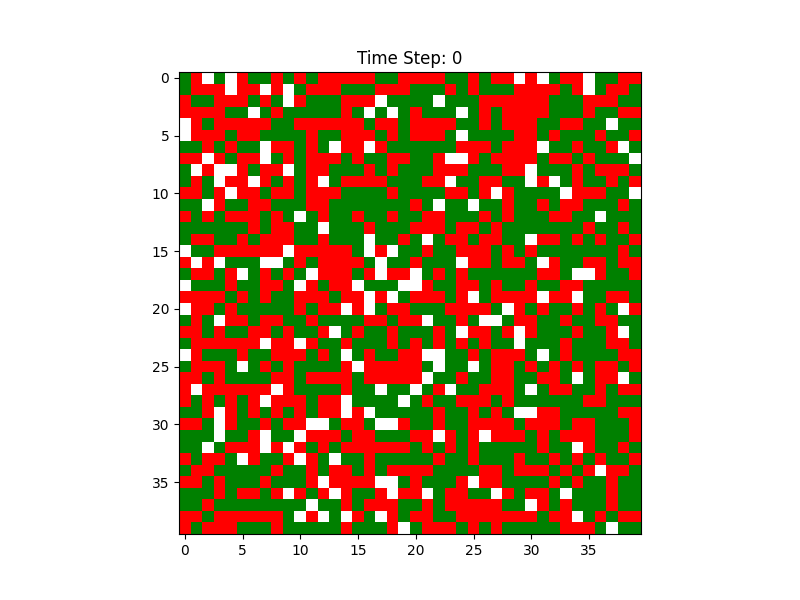
\includegraphics[width=\linewidth]{initial_random.png}
			\caption{\centering Random move}
		\end{subfigure}\hfill
		\begin{subfigure}{0.14\textwidth}
			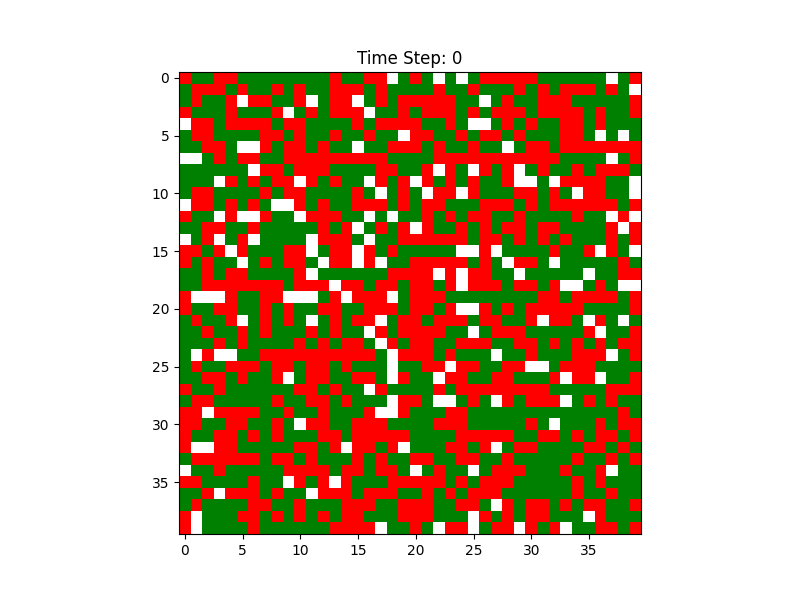
\includegraphics[width=\linewidth]{initial_social_n5p3.png}
			\caption{\centering SNR n=5, p=3}
		\end{subfigure}\hfill
		\begin{subfigure}{0.14\textwidth}
			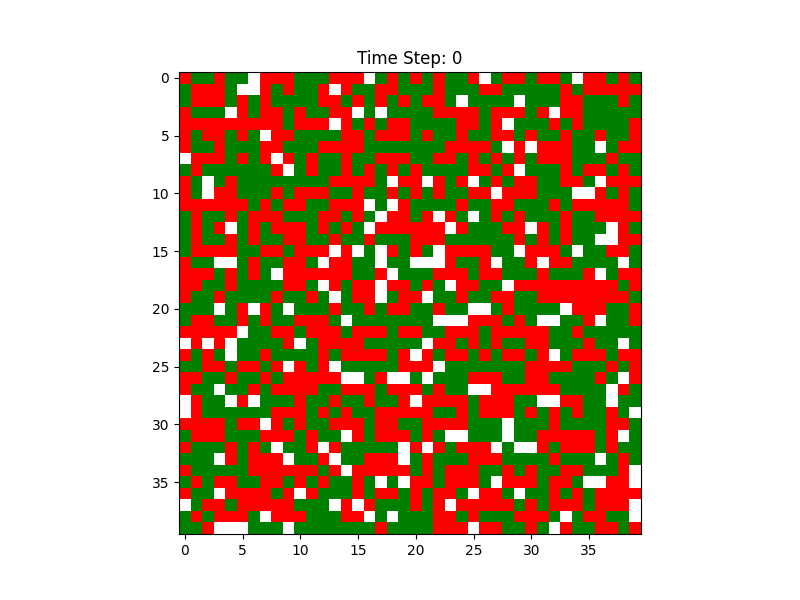
\includegraphics[width=\linewidth]{initial_social_n5p5.png}
			\caption{\centering SNR with n=5, p=5}
		\end{subfigure}\hfill
		\begin{subfigure}{0.14\textwidth}
			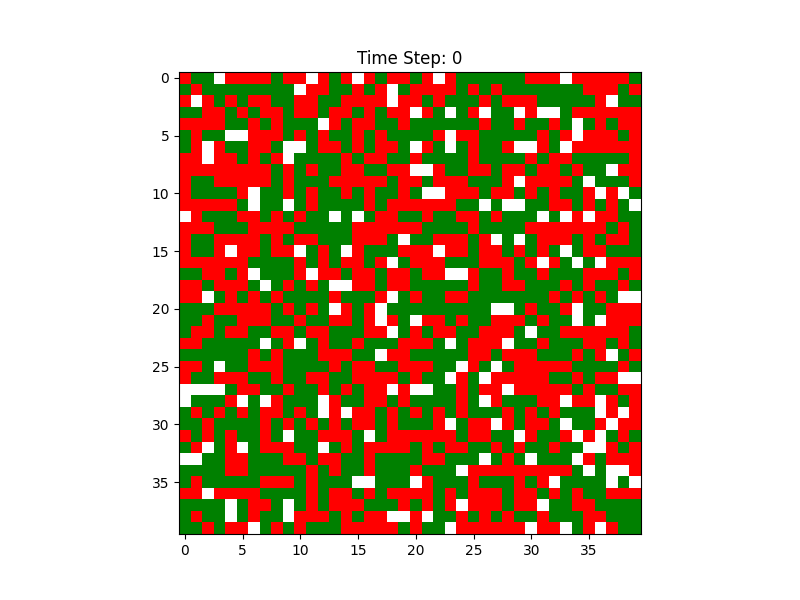
\includegraphics[width=\linewidth]{initial_social_n10p3.png}
			\caption{\centering SNR with n=10, p=3}
		\end{subfigure}\hfill
		\begin{subfigure}{0.14\textwidth}
			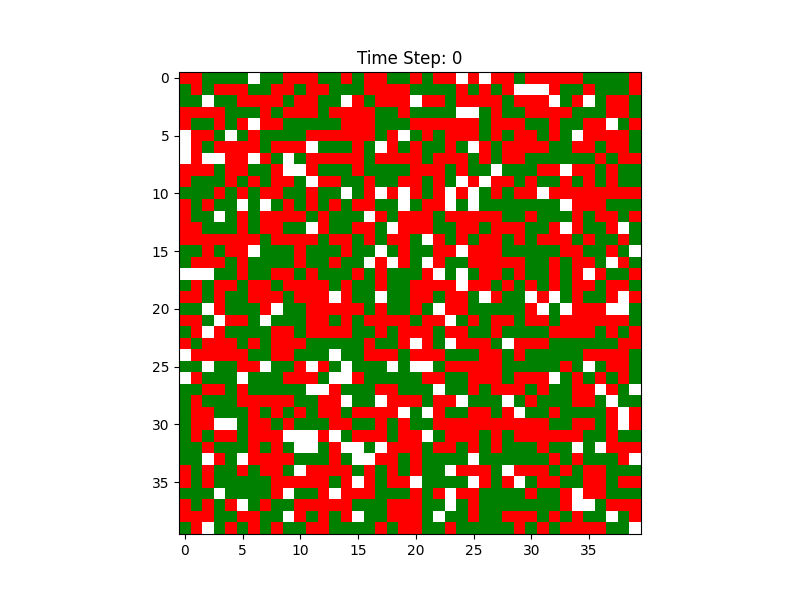
\includegraphics[width=\linewidth]{initial_social_n10p5.png}
			\caption{\centering SNR with n=10, p=5}
		\end{subfigure}\hfill
		\begin{subfigure}{0.14\textwidth}
			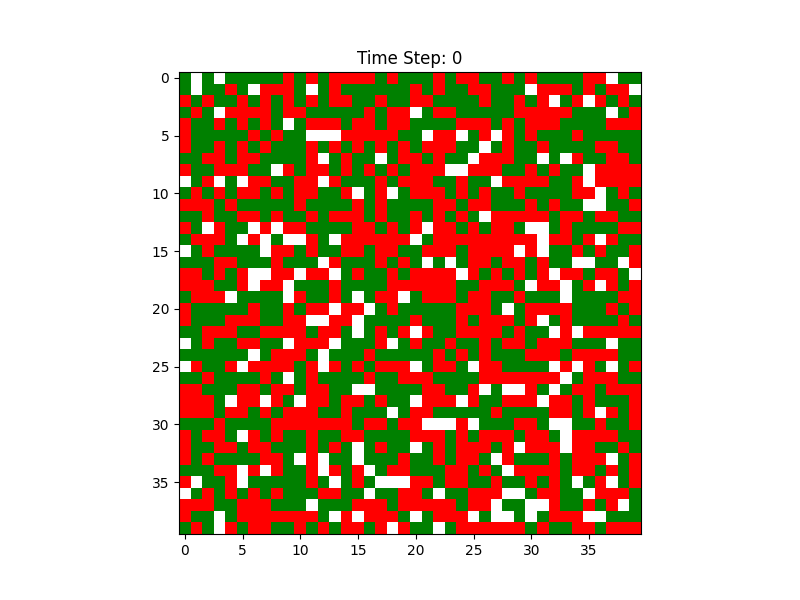
\includegraphics[width=\linewidth]{initial_social_n20p3.png}
			\caption{\centering SNR with n=20, p=3}
		\end{subfigure}\hfill
		\begin{subfigure}{0.14\textwidth}
			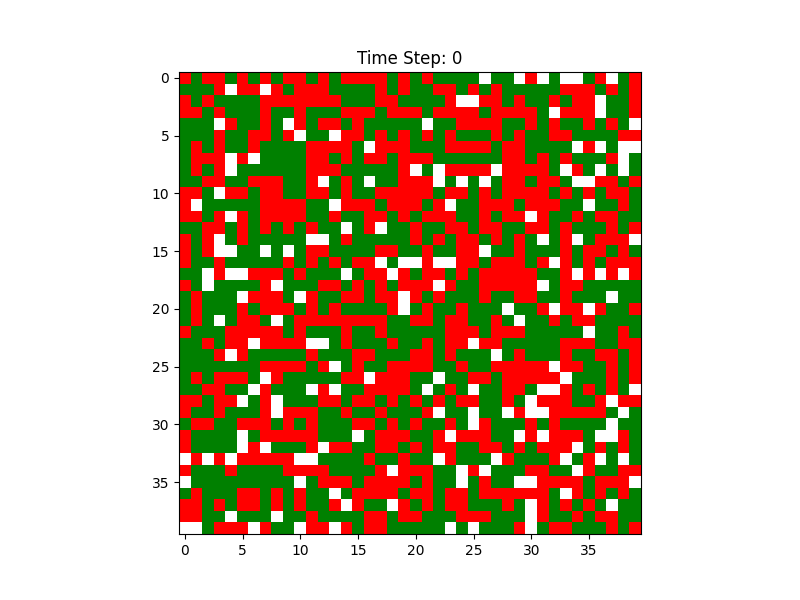
\includegraphics[width=\linewidth]{initial_social_n20p5.png}
			\caption{\centering SNR with n=20, p=5}
		\end{subfigure}
		\caption{Initial states for random move and social network recommendation policies}
	\end{figure}
	\vspace{-1em} % Adjust the vertical space here
	\begin{figure}[h]
		\centering
		\begin{subfigure}{0.14\textwidth}
			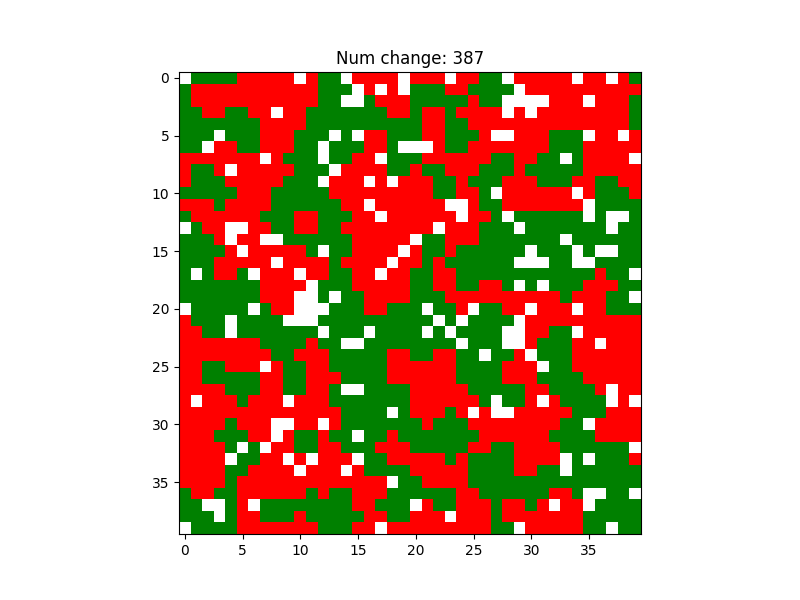
\includegraphics[width=\linewidth]{final_random.png}
			\caption{\centering Random move}
		\end{subfigure}\hfill
		\begin{subfigure}{0.14\textwidth}
			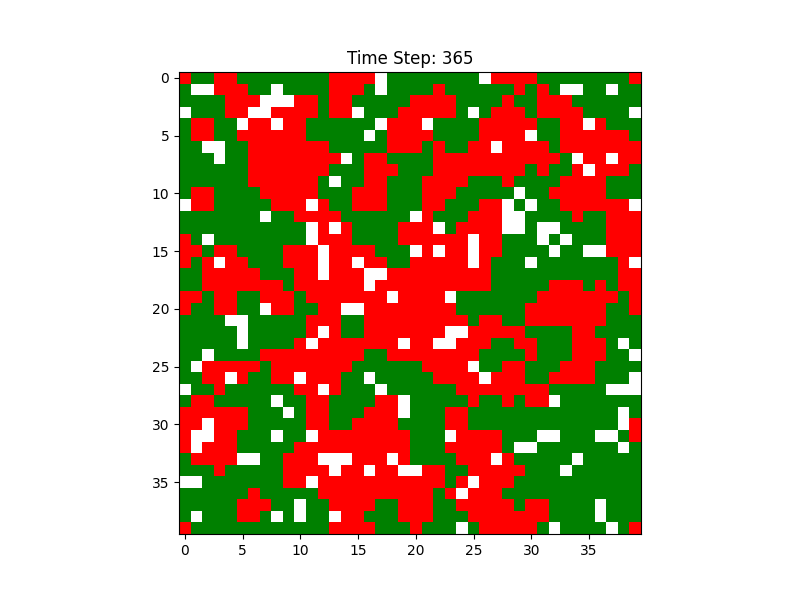
\includegraphics[width=\linewidth]{final_social_n5p3.png}
			\caption{\centering SNR with n=5, p=3}
		\end{subfigure}\hfill
		\begin{subfigure}{0.14\textwidth}
			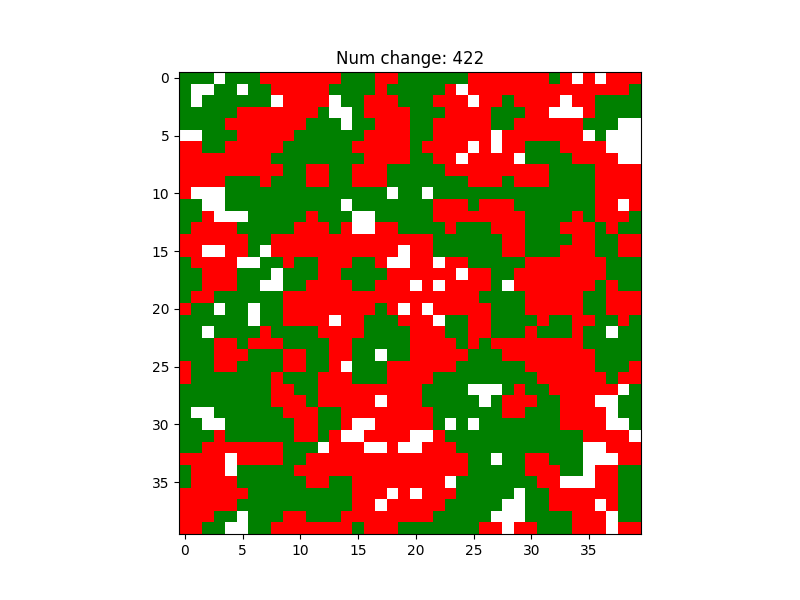
\includegraphics[width=\linewidth]{final_social_n5p5.png}
			\caption{\centering SNR with n=5, p=5}
		\end{subfigure}\hfill
		\begin{subfigure}{0.14\textwidth}
			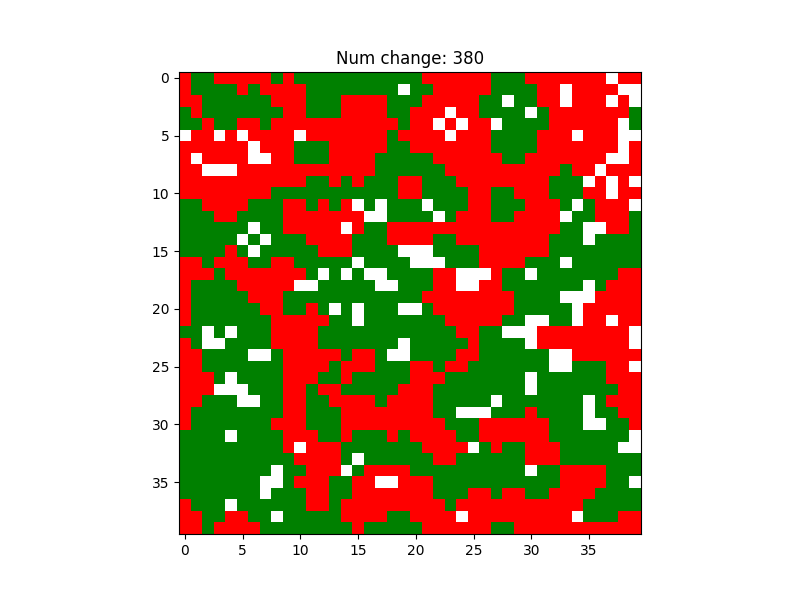
\includegraphics[width=\linewidth]{final_social_n10p3.png}
			\caption{\centering SNR with n=10, p=3}
		\end{subfigure}\hfill
		\begin{subfigure}{0.14\textwidth}
			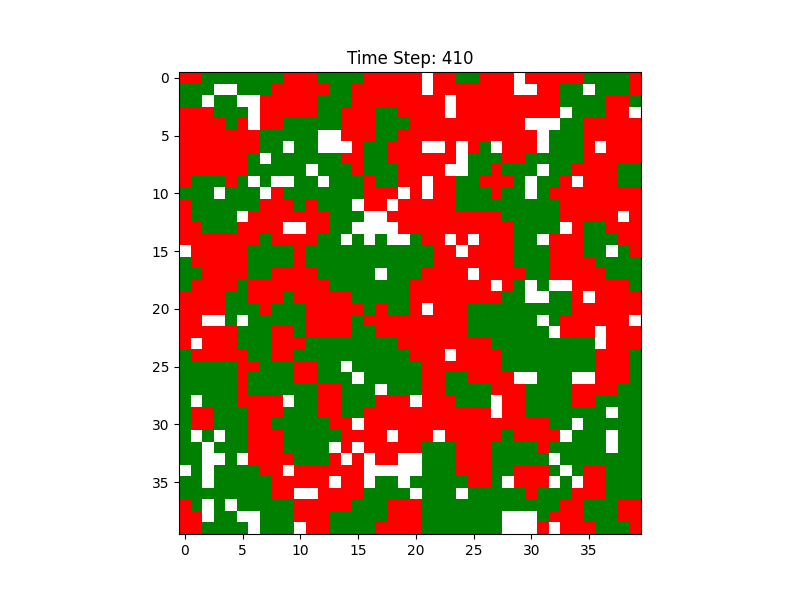
\includegraphics[width=\linewidth]{final_social_n10p5.png}
			\caption{\centering SNR with n=10, p=5}
		\end{subfigure}\hfill
		\begin{subfigure}{0.14\textwidth}
			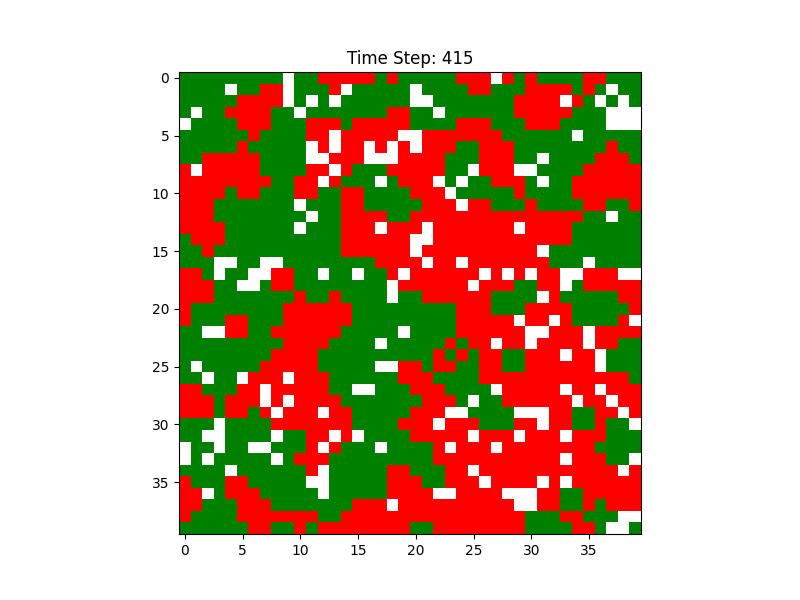
\includegraphics[width=\linewidth]{final_social_n20p3.png}
			\caption{\centering SNR with n=20, p=3}
		\end{subfigure}\hfill
		\begin{subfigure}{0.14\textwidth}
			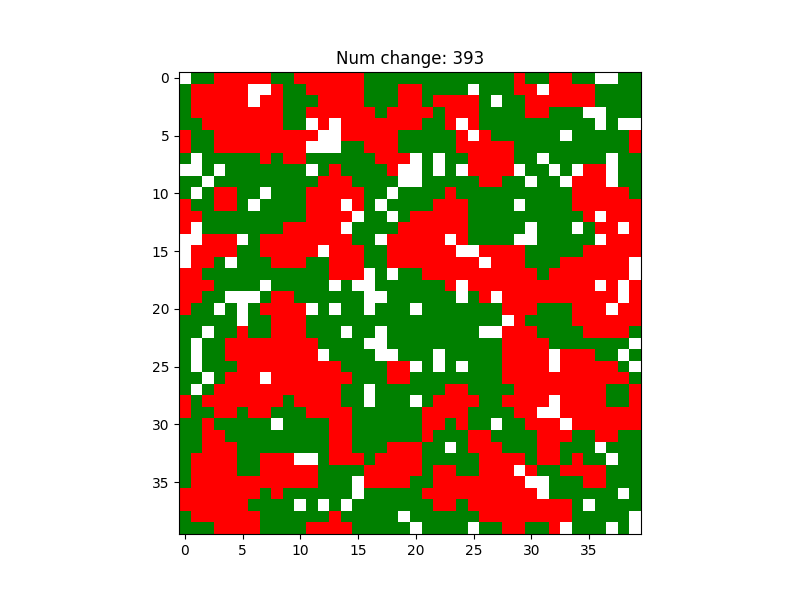
\includegraphics[width=\linewidth]{final_social_n20p5.png}
			\caption{\centering SNR with n=20, p=5}
		\end{subfigure}
		\caption{Final states of random move and social network recommendation policies}
	\end{figure}
	\vspace{-1em} % Adjust the vertical space here
	\begin{figure}[h]
		\centering
		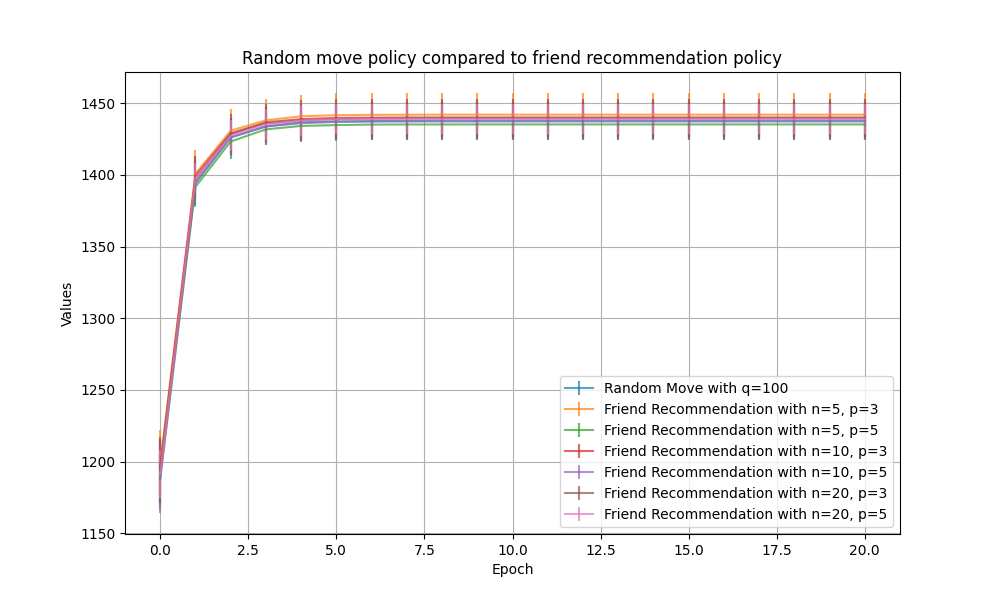
\includegraphics[width=\textwidth]{policies01.png}
		\caption{Time series comparing a random move policy with the social network recommendation policy}
	\end{figure}
	\FloatBarrier


	test test test


	\newpage
	\section{Section 2: Specialized Policies}
	\subsection{Rachael}
	\subsubsection{Policy Description}
	The segregation in housing application can be expanded to include searching within one's own neighborhood (SN) for a better house in the same area. The policy parameter $w$ defines the degree of separation from a neighbor, represented as the number of plots away from one's own plot the agent will travel to ask for recommendations and parameter $\beta$ defines the probability that a neighbor who is not the same type as the searcher is asked for available spots. This simulates asking neighbors of the same type in the area with a small chance of consulting neighbors of a different type. If none of the neighbors are aware of a good spot, the random move policy is applied. This policy is implemented as a BFS from the agent along matching agents up to the degree of separation limit.
	
	\subsubsection{Results}
	% for insertion of before/after plots
	\begin{figure}[h]
		\centering
		\begin{subfigure}{0.14\textwidth}
			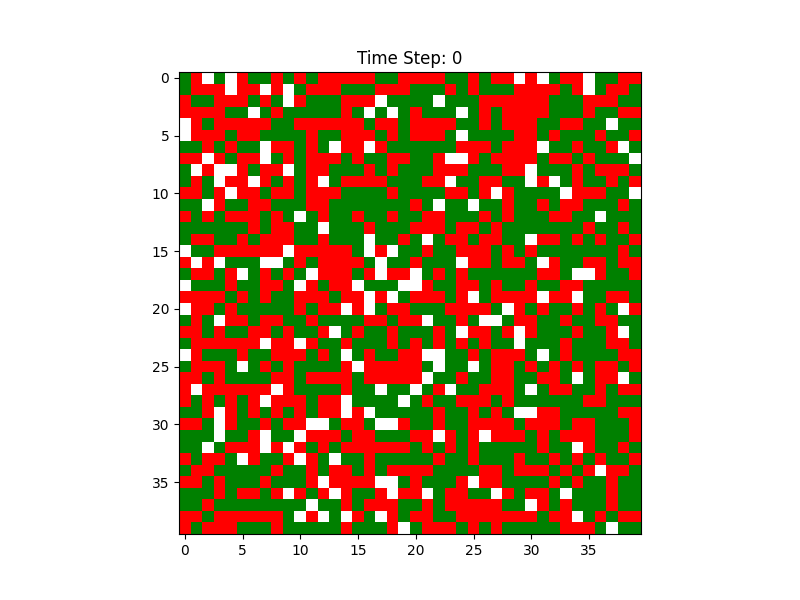
\includegraphics[width=\linewidth]{initial_random.png}
			\caption{\centering Random move}
		\end{subfigure}\hfill
		\begin{subfigure}{0.14\textwidth}
			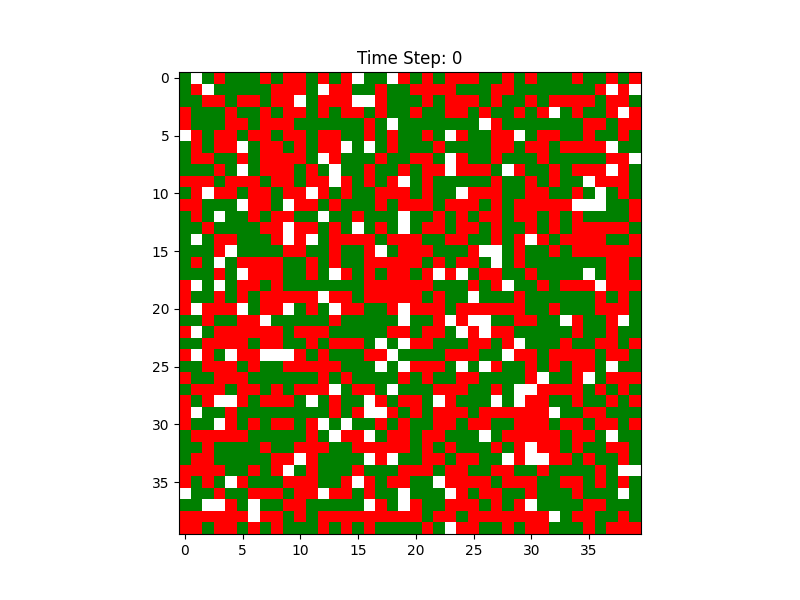
\includegraphics[width=\linewidth]{initial_cluster_w5b10.png}
			\caption{\centering SN w=5, beta=.1}
		\end{subfigure}\hfill
		\begin{subfigure}{0.14\textwidth}
			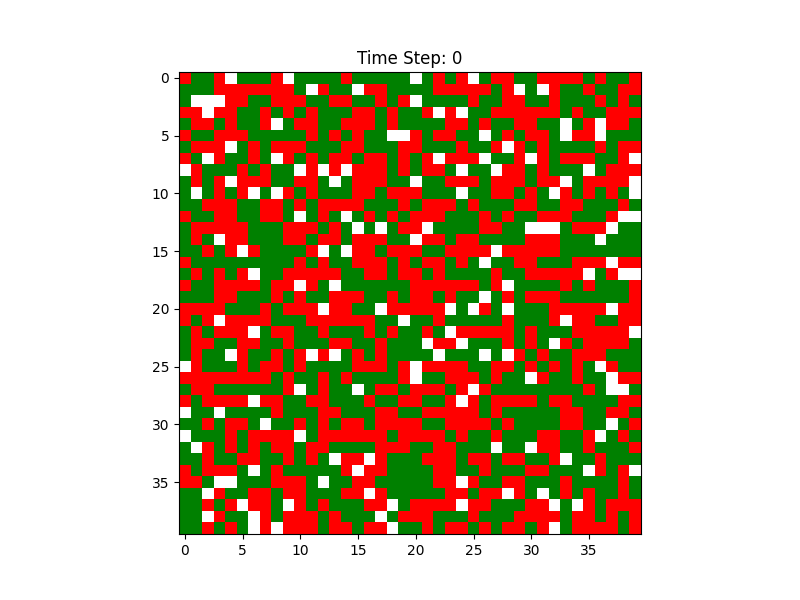
\includegraphics[width=\linewidth]{initial_cluster_w10b10.png}
			\caption{\centering SN w=10, beta=.1}
		\end{subfigure}\hfill
		\begin{subfigure}{0.14\textwidth}
			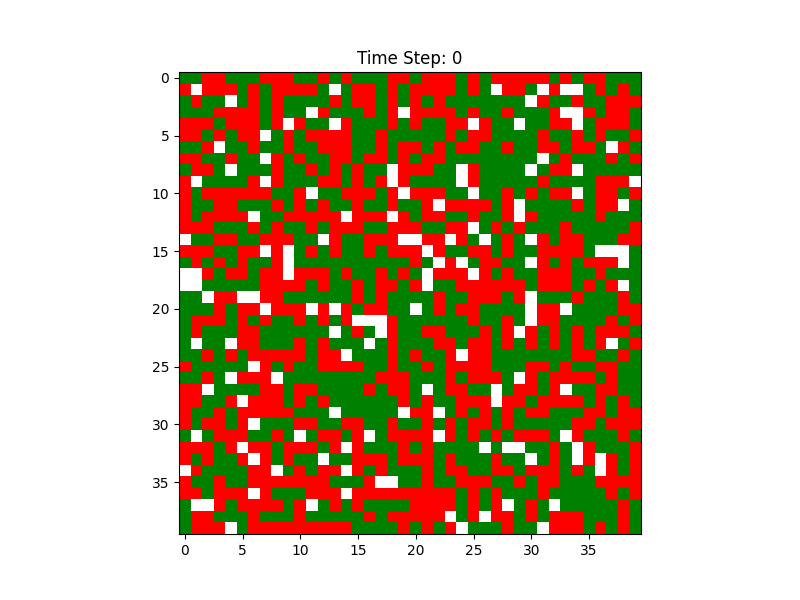
\includegraphics[width=\linewidth]{initial_cluster_w20b10.png}
			\caption{\centering SN w=20, beta=.1}
		\end{subfigure}\hfill
		\begin{subfigure}{0.14\textwidth}
			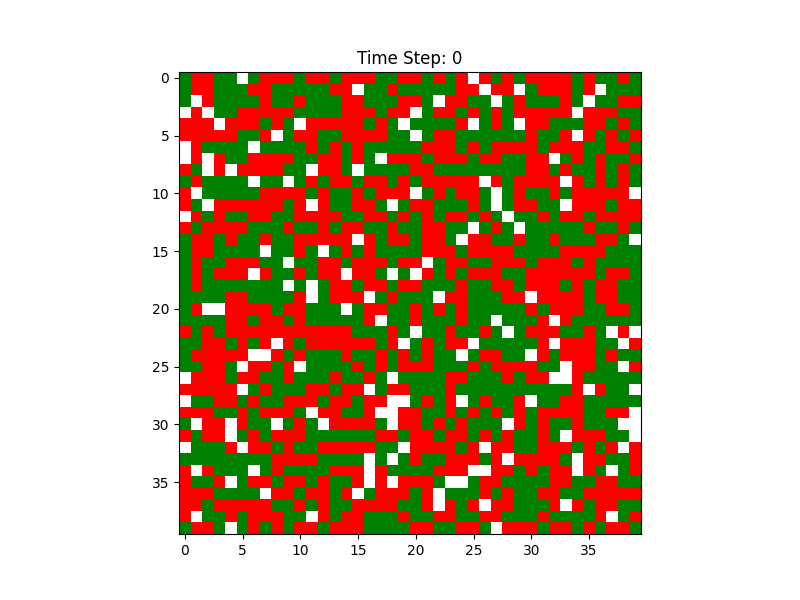
\includegraphics[width=\linewidth]{initial_cluster_w5b20.png}
			\caption{\centering SN w=5, beta=.2}
		\end{subfigure}\hfill
		\begin{subfigure}{0.14\textwidth}
			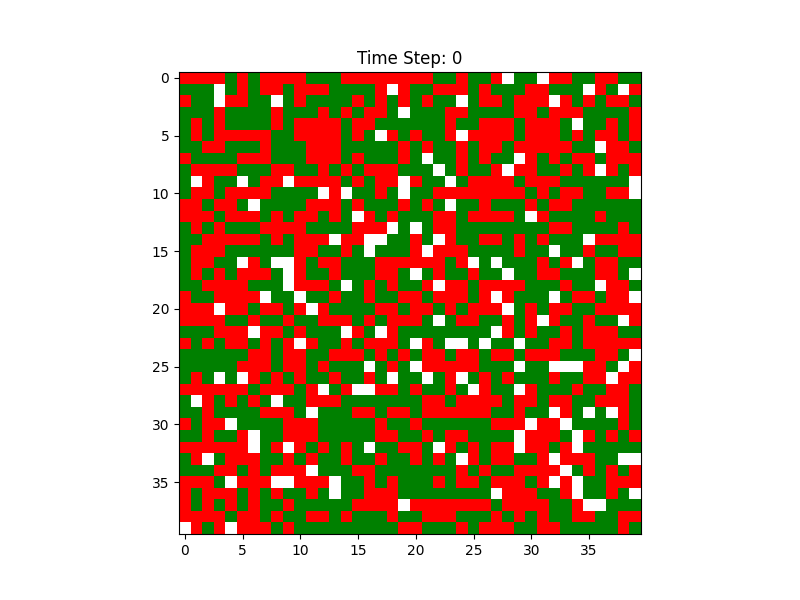
\includegraphics[width=\linewidth]{initial_cluster_w10b20.png}
			\caption{\centering SN w=10, beta=.2}
		\end{subfigure}\hfill
		\begin{subfigure}{0.14\textwidth}
			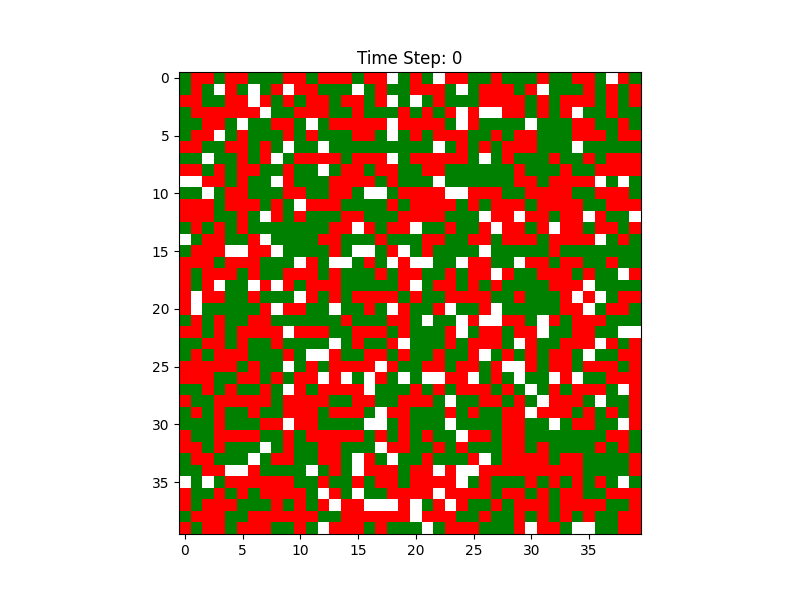
\includegraphics[width=\linewidth]{initial_cluster_w20b20.png}
			\caption{\centering SN w=20, beta=.2}
		\end{subfigure}
		\caption{Initial states of neighborhoods for random move and neighborhood search policy}
	\end{figure}
	\vspace{-2em} % Adjust the vertical space here
	\begin{figure}[h]
		\centering
		\begin{subfigure}{0.14\textwidth}
			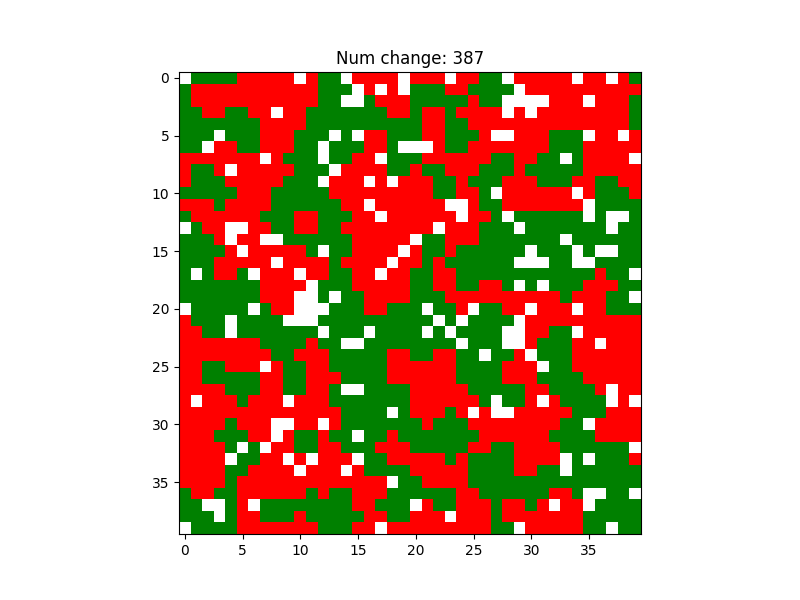
\includegraphics[width=\linewidth]{final_random.png}
			\caption{\centering Random move}
			\label{sn_finalrandom}
		\end{subfigure}\hfill
		\begin{subfigure}{0.14\textwidth}
			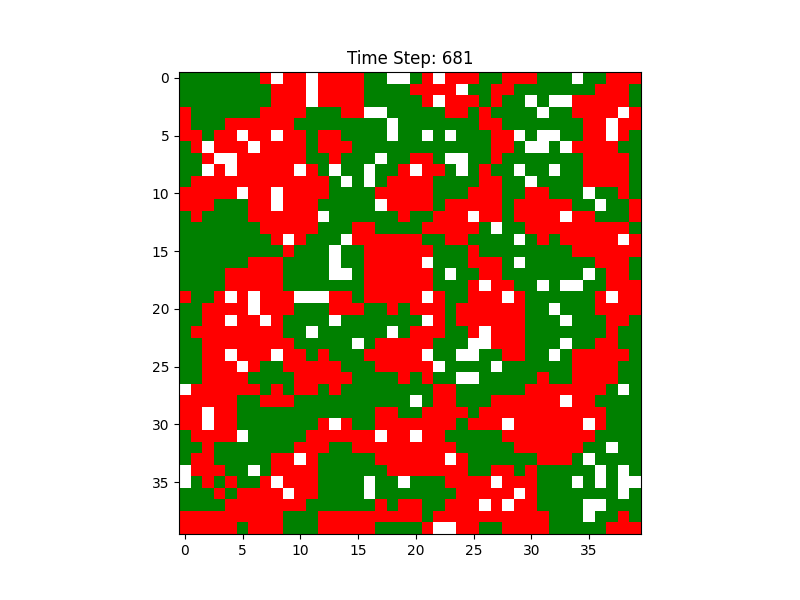
\includegraphics[width=\linewidth]{final_cluster_w5b10.png}
			\caption{\centering SN w=5, beta=.1}
			\label{sn_finalw5b10}
		\end{subfigure}\hfill
		\begin{subfigure}{0.14\textwidth}
			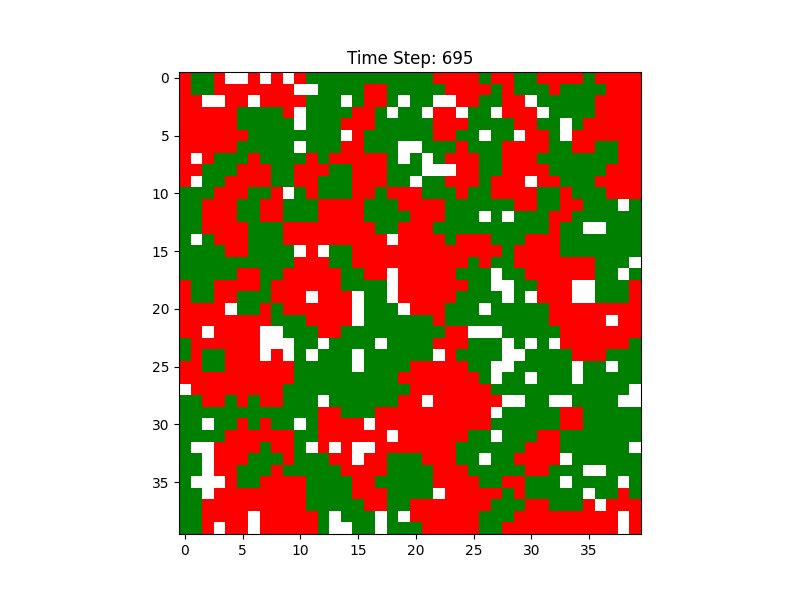
\includegraphics[width=\linewidth]{final_cluster_w10b10.png}
			\caption{\centering SN w=10, beta=.1}
			\label{sn_finalw10b10}
		\end{subfigure}\hfill
		\begin{subfigure}{0.14\textwidth}
			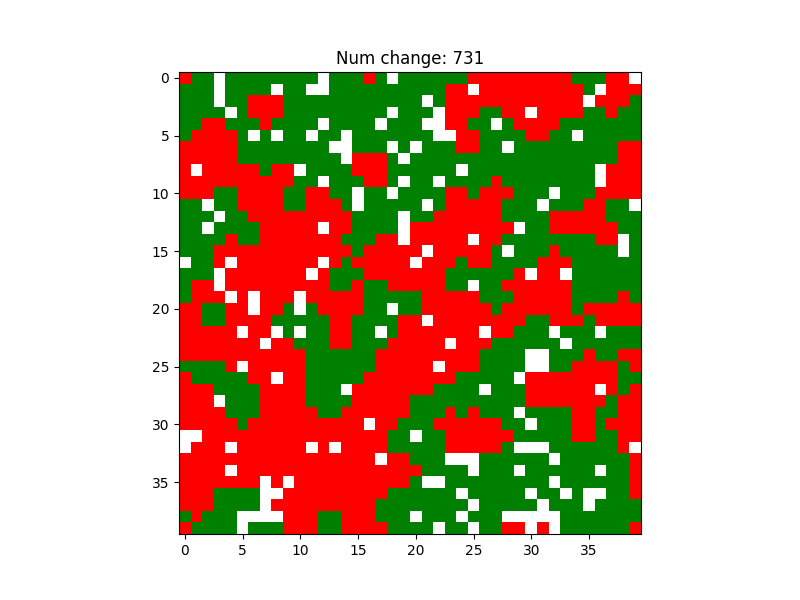
\includegraphics[width=\linewidth]{final_cluster_w20b10.png}
			\caption{\centering SN w=20, beta=.1}
			\label{sn_finalw20b10}
		\end{subfigure}\hfill
		\begin{subfigure}{0.14\textwidth}
			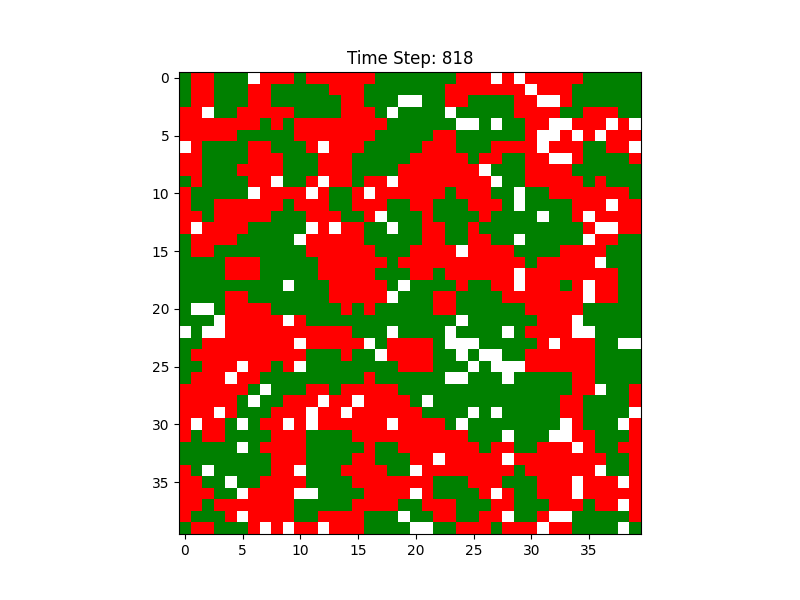
\includegraphics[width=\linewidth]{final_cluster_w5b20.png}
			\caption{\centering SN w=5, beta=.2}
			\label{sn_finalw5b20}
		\end{subfigure}\hfill
		\begin{subfigure}{0.14\textwidth}
			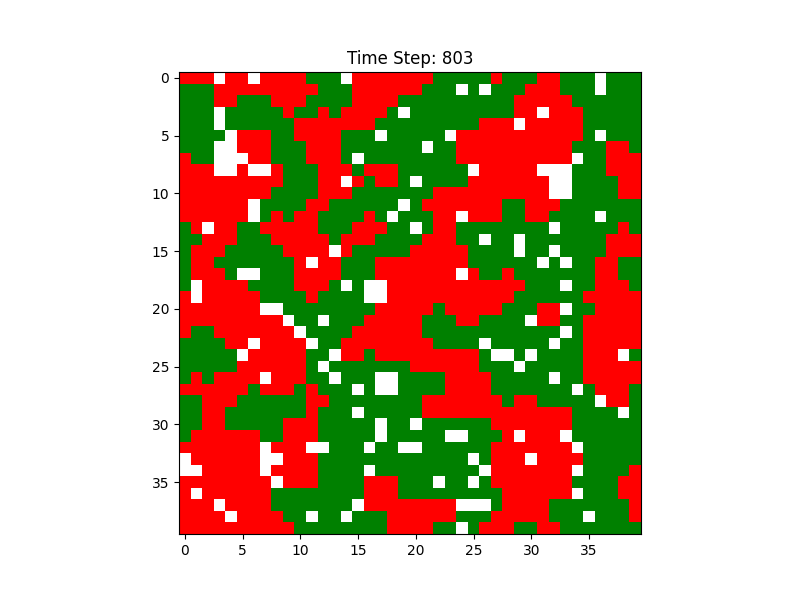
\includegraphics[width=\linewidth]{final_cluster_w10b20.png}
			\caption{\centering SN w=10, beta=.2}
			\label{sn_finalw10b20}
		\end{subfigure}\hfill
		\begin{subfigure}{0.14\textwidth}
			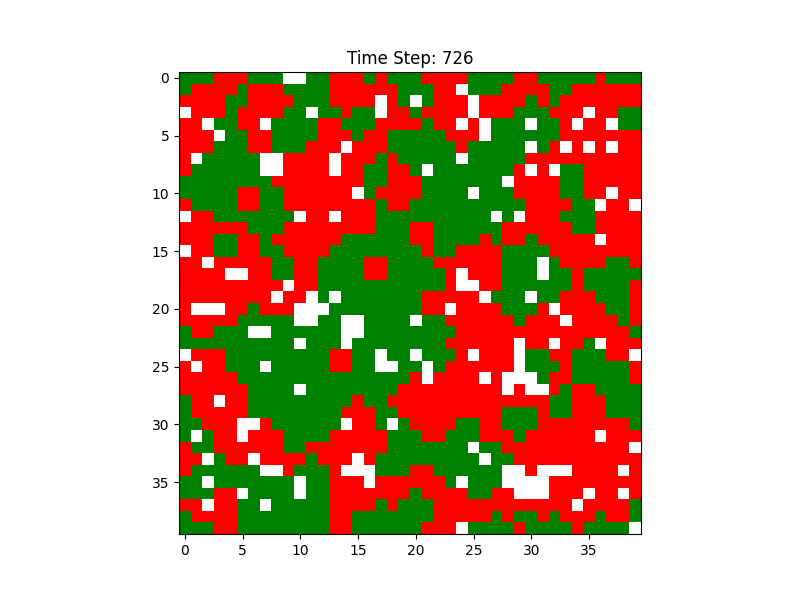
\includegraphics[width=\linewidth]{final_cluster_w20b20.png}
			\caption{\centering SN w=20, beta=.2}
			\label{sn_finalw20b20}
		\end{subfigure}
		\caption{Final states for random move and neighborhood search policies}
		\label{sn_finalstate}
	\end{figure}
	\FloatBarrier
	
	\begin{wrapfigure}{l}{.5\textwidth}
		\centering
		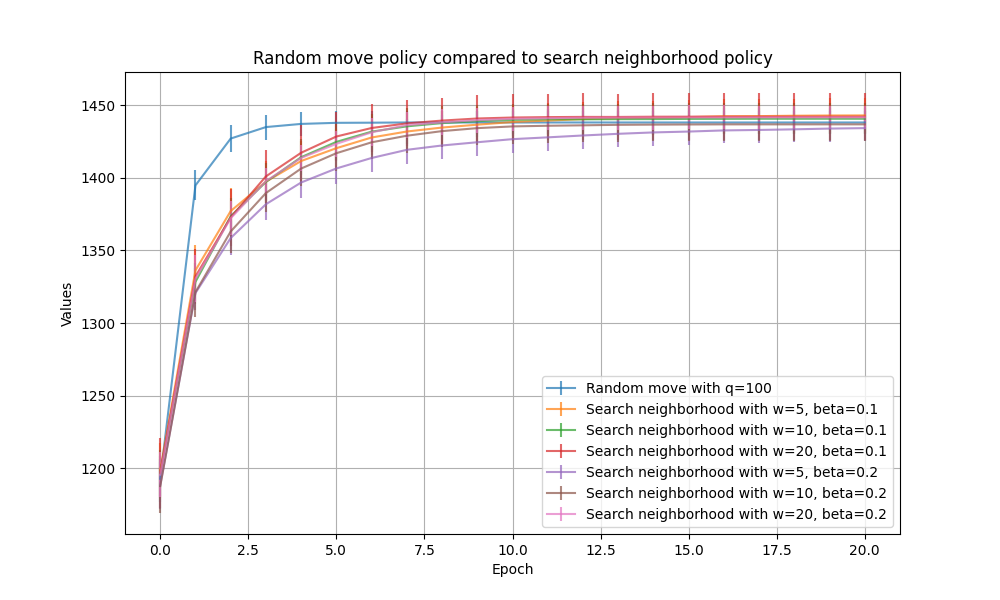
\includegraphics[width=.5\textwidth]{policies02.png}
		\caption{Time series comparison of neighborhood search compared to random move}
	\end{wrapfigure}
	This policy resulted in fully connected clusters across the map of like agents in Fig \ref{sn_finalstate}. The exceptions are clusters of four agents (see Fig \ref{sn_finalw20b20}), which meet the k=3 requirement while being small enough to not connect to the main cluster. Further, due to the search only of neighboring spaces, when a cluster of empty spaces appears, it often remains open because its plots are never reported by neighbors, despite partial happiness for nearby empty plots as well as agents getting stuck until they talk to a mismatched neighbor. This method results in a slower convergence to optimal happiness but ends up better than the random move search as happy neighborhoods form. The neighborhood search with smaller separation with lower probability of talking to mismatched neighbors produced the highest overall average happiness of the automata (ie, talking primarily to neighbors of the same type). This is perhaps because it makes the agent remain in its own cluster of like agents instead of hopping between  clusters as could occur with a greater $w$. The standard deviations were all wide enough to include the happiness of the other parameter configurations so  conclusions have a margin for error.
	
	\newpage
	
	\subsection{Connor}
	
	
	
	
	\newpage
	
	\subsection{Josh}
	
	


	
\end{document}